%% 
%% Copyright 2019-2020 Elsevier Ltd
%% 
%% This file is part of the 'CAS Bundle'.
%% --------------------------------------
%% 
%% It may be distributed under the conditions of the LaTeX Project Public
%% License, either version 1.2 of this license or (at your option) any
%% later version.  The latest version of this license is in
%%    http://www.latex-project.org/lppl.txt
%% and version 1.2 or later is part of all distributions of LaTeX
%% version 1999/12/01 or later.
%% 
%% The list of all files belonging to the 'CAS Bundle' is
%% given in the file `manifest.txt'.
%% 
%% Template article for cas-dc documentclass for 
%% double column output.

%\documentclass[a4paper,fleqn,longmktitle]{cas-dc}
\documentclass[a4paper,fleqn]{cas-sc}

%\usepackage[numbers]{natbib}
%\usepackage[authoryear]{natbib}
\usepackage[authoryear,longnamesfirst]{natbib}
\usepackage{graphicx}
\usepackage{caption}
\usepackage{subcaption}
\usepackage{booktabs}
\usepackage{longtable}

%%%Author definitions
\def\tsc#1{\csdef{#1}{\textsc{\lowercase{#1}}\xspace}}
\tsc{WGM}
\tsc{QE}
\tsc{EP}
\tsc{PMS}
\tsc{BEC}
\tsc{DE}
%%%

% Uncomment and use as if needed
%\newtheorem{theorem}{Theorem}
%\newtheorem{lemma}[theorem]{Lemma}
%\newdefinition{rmk}{Remark}
%\newproof{pf}{Proof}
%\newproof{pot}{Proof of Theorem \ref{thm}}

\begin{document}
\let\WriteBookmarks\relax
\def\floatpagepagefraction{1}
\def\textpagefraction{.001}

% Short title
\shorttitle{Correspondence Analysis of Two-Mode Networks}

% Short author
%\shortauthors{O. Lizardo}

% Main title of the paper
\title [mode = title]{The Correspondence Analysis of Two-Mode Networks Revisited}                      
% Title footnote mark
% eg: \tnotemark[1]
%\tnotemark[1,2]

% Title footnote 1.
% eg: \tnotetext[1]{Title footnote text}
% \tnotetext[<tnote number>]{<tnote text>} 
%\tnotetext[1]{}

%\tnotetext[2]{.}


% First author
%
% Options: Use if required
% eg: \author[1,3]{Author Name}[type=editor,
%       style=chinese,
%       auid=000,
%       bioid=1,
%       prefix=Sir,
       %orcid=0000-0002-5405-3007,
%       facebook=<facebook id>,
%       twitter=<twitter id>,
%       linkedin=<linkedin id>,
%       gplus=<gplus id>]
%\author[1]{Omar Lizardo}[orcid=0000-0002-5405-3007]

% Corresponding author indication
%\cormark[1]

% Footnote of the first author
%\fnmark[1]

% Email id of the first author
%\ead{olizardo@soc.ucla.edu}

% URL of the first author
%\ead[url]{http://olizardo.bol.ucla.edu/}

%  Credit authorship
%\credit{Conceptualization of this study, Methodology, Software}

%Address/affiliation
%\affiliation[1]{organization={University of California, Los Angeles},
   % addressline={264 Haines Hall}, 
   % city={Los Angeles},
    %citysep={},  Uncomment if no comma needed between city and postcode
    % postcode={90095}, 
    % state={CA},
    % country={USA}}

 %Corresponding author text
%\cortext[cor1]{Corresponding author}
%\cortext[cor2]{Principal corresponding author}

%Footnote text
%\fntext[fn1]{This paper was written while the author was partially supported by National Science Foundation grant HNDS-R \#2214215.}
 % author as well.}
%\fntext[fn2]{Another author footnote, this is a very long footnote and
 % it should be a really long footnote. But this footnote is not yet
 % sufficiently long enough to make two lines of footnote text.}

% For a title note without a number/mark
%\nonumnote{This note has no numbers. In this work we demonstrate $a_b$
%  the formation Y\_1 of a new type of polariton on the interface
 % between a cuprous oxide slab and a polystyrene micro-sphere placed
 % on the slab.
 % }
% Here goes the abstract
\begin{abstract}
This paper reconsiders the use of Correspondence Analysis (CA) in analyzing two-mode network data, highlighting aspects that have not been previously emphasized, going beyond the use of CA as a visualization tool. It argues that CA can be used to compute a dual centrality score on both modes, related to but not mathematically equivalent to the \citet{bonacich1991simultaneous} two-mode centrality. This ``reflective'' centrality score connects the use of CA in two-mode network analysis to its use in other disciplines as a method of ordination. Additionally, I show CA can extract latent positional information on people and groups, with similarities to recent work on ``generalized relational similarity" in two-mode networks. Thus, CA can be used for indirect community or subgroup identification in two-mode networks, connecting to its use in some disciplines as a clustering method. The paper demonstrates these applications of CA, comparing them with the Bonacich dual centrality scores, and provides guidance on using CA for structural analysis in network analysis.
\end{abstract}

% Use if graphical abstract is present
% \begin{graphicalabstract}
% \includegraphics{figs/grabs.pdf}
% \end{graphicalabstract}

%Research highlights
\begin{highlights}
  \item This paper revisits the use of Correspondence Analysis (CA) in analyzing two-mode network data, highlighting its potential beyond data visualization.
  \item CA can compute a dual centrality score on both modes of a two-mode network, related to but not mathematically equivalent to the Bonacich (1991) two-mode centrality. 
  \item CA can extract latent positional information on people and groups, with similarities to recent work on generalized relational similarity" in two-mode networks. 
\end{highlights}

% Keywords
% Each keyword is separated by \sep
\begin{keywords}
Correspondence Analysis \sep Generalized Relational Similarity \sep Duality \sep Two-mode networks \sep Centrality 
\end{keywords}

\maketitle
\newpage
\section{Introduction} \label{sec:intro}
While not particularly common, using Correspondence Analysis---hereafter CA---in analyzing two-mode network data has had a somewhat rocky career in the social networks literature. Initially criticized by \citet{borgatti1997network} as a relatively limited and perhaps even inapplicable tool, CA has found various proponents who see it as an important component of the SNA arsenal for two-mode network data analysis, particularly regarding its ability to economically provide synoptic (e.g., ``joint'') graphical representations of structural connectivity patterns across the two-modes \citep{roberts2000correspondence, breiger2000tool, faust2005using}, with the primary aim being to use CA---or its variants like Multiple Correspondence Analysis (MCA)---to ``visually explore'' such networks \citep{d2014use}. This paper contributes to the stream of previous work applying CA to analyze two-mode data. Nevertheless, it departs from the already-mentioned previous efforts in highlighting aspects of CA for two-mode data analysis in SNA that have not been emphasized or treated in detail before, moving beyond the focus on data visualization. 

Particularly, I show that CA can be thought of as computing a kind of \textit{dual centrality} score on both modes---one related to but not mathematically equivalent to the Bonacich \citeyearpar{bonacich1991simultaneous} two-mode centrality----an approach that, as noted by \citet{van2021correspondence}, has been recently re-invented in some corners of network science under the guise of the ``economic complexity index'' \citep{hidalgo2009building, mealy2019interpreting}. With \citet{van2021correspondence}, I argue that this is a rather restricted interpretation of a more general centrality score connecting the use of CA in two-mode network analysis to way CA features in some disciplines also concerned with two-mode data (e.g., ecology) as a method of \textit{ordination}---e.g., the discovery of latent one-dimensional orderings among a set of entities. In social network analysis, this applies to conceptualizing the venerable duality between people and the groups they join \citep{breiger1974duality}.

In addition to its capacity to reveal latent ordinal structure in two-mode data, I also argue that CA can also be used to extract latent \textit{positional} information on people and groups. Particularly, there is a suggestive similarity between the scores obtained from the first dimension of the CA of the two-mode affiliation matrix (the aforementioned dual centrality score) and recent work on ``generalized relational similarity'' in two-mode networks \citep{kovacs2010generalized, lizardo2024two}. As such, CA recovers clusters of entities (e.g., people) linked by their similar connectivity patterns to similar entities in the other mode (e.g., groups). Thus, CA can be used as an approach to indirect ``community'' identification in two-mode networks connecting to how CA is used in some disciplines (e.g., computer and information science) as a \textit{clustering} method \citep{zha2001bipartite}, namely, the discovery of sociometrically similar subsets of entities in affiliation networks. In this way, CA emerges as a tool central to the usual network-analytic tasks and not just as a visualization or data-summarization tool.

\subsection{Organization of the Paper} \label{subsec:org}
The rest of the paper is organized as follows. In the next section, I motivate the use of CA as producing a type of Bonacich-style dual centrality via weighted iteration across the two modes of the affiliation matrix. This leads naturally to an abbreviated way of computing the same scores via eigenvector decomposition of the (inverse degree-weighted) one-mode projection of the affiliation matrix for each set of nodes. This approach is computationally and mathematically related but \textit{not} equivalent to the eigenvalue decomposition of the one-mode projection matrices, which results in the usual Bonacich dual centrality scores. I then draw on recent work by \citet{van2021correspondence} to show the links between the ordering of nodes along the first CA dimension and Kovacs's generalized relational similarity, and the distance of nodes in the space formed by the first two dimensions and the connectivity-similarity between nodes across modes. I contrast this ordering to that provided by the Bonacich dual centrality scores, which in contrast to the CA ordering---which reveals a dual community partition--- recovers the core-periphery structure of the two-mode network instead. In closing, I provide some pointers on how CA can be used as a method for structural (e.g., centrality and positional) analysis, independently of the usual emphasis on joint graphical displays and visual exploration. 

\section{Reflective Centralities in Two-Mode Networks} \label{sec:ref2mode}
In a highly cited piece, \citet{hidalgo2009building} motivated what they saw at the time as a novel way of ranking nodes in a two-mode network---effectively computing a version of two-mode centrality---using what they called at the time a ``reflective'' approach. Hidalgo and Hausmann's original empirical application was to the two-mode country-by-product networks, hence the original baptizing of their approach as one geared to extracting the ``economic complexity'' of countries in the world system (and dually the complexity of given products). Subsequent work shows that there is no logical connection between the formal method and this particular application since the approach proposed can be used to analyze any two-mode data matrix. As such, I introduce it here using the more intuitive---and classical from a social network analysis perspective---case of the duality of persons and groups \citep{breiger1974duality}. 

If we are going to compute the centrality of nodes in a two-mode network, the most natural place to start is with the good old \textit{degree centrality} \citep{faust1997centrality}. A two-mode network composed of a set of people $P$ and their affiliation relations to a set of groups $G$ can be represented by an affiliation matrix $\mathbf{A}$ of dimensions $|P| \times |G|$ with people along the rows and groups across the columns, where $|P|$ is the cardinality of the people set and $|G|$ is the cardinality of the group set, with cell entries $a_{pg}= 1$ if person \textit{p} is affiliated with group \textit{g} and $a_{pg}= 0$ otherwise. 

Given this, the degree-centrality of people is given by:

\begin{equation}
    C^R_p(1) = \sum_g a_{pg}
    \label{eq:R1_p}
\end{equation}

And for groups:

\begin{equation}
   C^R_g(1) = \sum_p a_{pg}
  \label{eq:R1_g}
\end{equation}

That is, the first-order centrality of people is the row sum of the entries in the affiliation matrix $A$, and the column sums of the same matrix give the first-order centrality of groups. As noted by \citet{hidalgo2009building}, the key to the reflective approach is the observation that, once we have these first-order quantities, it is possible to compute ``second-order centralities'' $C^R(2)$ for both people and groups using the (averaged) first-order centralities of the entities in the other mode they are connected to. 

For people, these are given by:

\begin{equation}
    C^R_p(2) = \frac{1}{C^R_p(1)}\sum_g a_{pg}C^R_g(1)
    \label{eq:R2_p}
\end{equation}

And for groups:

\begin{equation}
   C^R_g(2) = \frac{1}{C^R_g(1)}\sum_p a_{pg}C^R_p(1)
    \label{eq:R2_g}
\end{equation}

Equation \ref{eq:R2_p} says ``people are more central when the average sum of the size of the groups they belong to is large'' (e.g., whenever $a_{pg} = 1$ and $C^R_g(1)$ is a big number). Equation \ref{eq:R2_g} says ``groups are more central when the average activity of their members is large'' (e.g., whenever $a_{pg} = 1$ and $C^R_p(1)$ is a big number). Of course, we can keep on going and define third-order reflections. 

For the people, these are given by:

\begin{equation}
   C^R_p(3) = \frac{1}{C^R_p(1)}\sum_g a_{pg}C^R_g(2)
   \label{eq:R3_p}
\end{equation}

And for groups:

\begin{equation}
   C^R_g(3) = \frac{1}{C^R_g(1)}\sum_p a_{pg}C^R_p(2)
   \label{eq:R3_g}
\end{equation}

Equation \ref{eq:R3_p} says something like ``people are more central when the average sum of the average activity of the members of the groups they belong to is large'' (e.g., $a_{pg} = 1$ and $C^R_g(2)$ is a big number). Equation \ref{eq:R3_g} says, ''groups are more central when the average sum of the average size of the groups their members belong to is large.'' (e.g., $a_{pg} = 1$ and $C^R_p(2)$ is a big number).

Note that for the people, the even-numbered reflection $C^R_p(2)$ assigns centrality based on a formal feature of the \textit{groups} they belong to (in this case, the group sizes). On the other hand, the odd-numbered reflection $C^R_p(3)$ assigns centrality based on a formal feature of the \textit{members of the groups} they belong to (in this case, the average size of the groups they belong to). In the same way, for the groups, the even-numbered reflection $C^R_g(2)$ assigns centrality based on a formal feature of the \textit{people} who belong to them (in this case, their activity). On the other hand, the odd-numbered reflection $C^R_g(3)$ assigns centrality based on a formal feature of the \textit{other groups their members belong to} (in this case, their average group size). While these are distinct metrics, in practice, the ordering of the nodes in each mode ends up being identical across even and odd centralities after the ranks ``freeze'' past a given number of iterations (proportional to the network size). 

More generally, \citet{hidalgo2009building} show that we can define a series of reflective quantities for people and groups (whose verbal and substantive interpretation becomes more complex as the number of iterations increases). 

For people, these are given by:

\begin{equation}   
    C^R_p(q) = \frac{1}{C^R_p(1)}\sum_g a_{pg}C^R_g(q-1) 
   \label{eq:Rq_p}
\end{equation}

And for groups:

\begin{equation}
   C^R_g(q) = \frac{1}{C^R_g(1)}\sum_p a_{pg}C^R_p(q-1)
   \label{eq:Rq_g}
\end{equation}

Equation~\ref{eq:Rq_p} says that the reflective centrality of a person \textit{p} at iteration \textit{q} is the sum of the $q-1$ centralities of the groups they belong to ($C^R_g(q-1)$) divided by their number of memberships $C^{R}_p(1)$. Equation~\ref{eq:Rq_g} says that the $q^{th}$ group reflective centrality is the sum of $q-1$ centralities $C^R_p(q-1)$ of their members, divided by the number of group members $C^R_g(1)$.

\begin{table}
\caption{Southern Women Data.}
\label{tab:southern}
\begin{tabular}[]{lcccccccccccccc}
\hline
 & E1 & E2 & E3 & E4 & E5 & E6 & E7 & E8 & E9 & E10 & E11 & E12 & E13 & E14 \\
 \hline
EVELYN & 1 & 1 & 1 & 1 & 1 & 1 & 0 & 1 & 1 & 0 & 0 & 0 & 0 & 0 \\
LAURA & 1 & 1 & 1 & 0 & 1 & 1 & 1 & 1 & 0 & 0 & 0 & 0 & 0 & 0 \\
THERESA & 0 & 1 & 1 & 1 & 1 & 1 & 1 & 1 & 1 & 0 & 0 & 0 & 0 & 0 \\
BRENDA & 1 & 0 & 1 & 1 & 1 & 1 & 1 & 1 & 0 & 0 & 0 & 0 & 0 & 0 \\
CHARLOTTE & 0 & 0 & 1 & 1 & 1 & 0 & 1 & 0 & 0 & 0 & 0 & 0 & 0 & 0 \\
FRANCES & 0 & 0 & 1 & 1 & 1 & 1 & 0 & 1 & 0 & 0 & 0 & 0 & 0 & 0 \\
ELEANOR & 0 & 0 & 0 & 1 & 1 & 1 & 1 & 1 & 0 & 0 & 0 & 0 & 0 & 0 \\
RUTH & 0 & 0 & 0 & 1 & 1 & 0 & 1 & 1 & 1 & 0 & 0 & 0 & 0 & 0 \\
VERNE & 0 & 0 & 0 & 0 & 0 & 0 & 1 & 1 & 1 & 0 & 0 & 1 & 0 & 0 \\
MYRA & 0 & 0 & 0 & 0 & 0 & 0 & 0 & 1 & 1 & 1 & 0 & 1 & 0 & 0 \\
KATHERINE & 0 & 0 & 0 & 0 & 0 & 0 & 0 & 1 & 1 & 1 & 0 & 1 & 1 & 1 \\
SYLVIA & 0 & 0 & 0 & 0 & 0 & 0 & 1 & 1 & 1 & 1 & 0 & 1 & 1 & 1 \\
NORA & 0 & 0 & 0 & 0 & 0 & 0 & 1 & 0 & 1 & 1 & 1 & 1 & 1 & 1 \\
HELEN & 0 & 0 & 0 & 0 & 0 & 0 & 1 & 1 & 0 & 1 & 1 & 1 & 0 & 0 \\
OLIVIA & 0 & 0 & 0 & 0 & 0 & 0 & 0 & 0 & 1 & 0 & 1 & 0 & 0 & 0 \\
FLORA & 0 & 0 & 0 & 0 & 0 & 0 & 0 & 0 & 1 & 0 & 1 & 0 & 0 & 0 \\
PEARL & 0 & 0 & 0 & 0 & 0 & 1 & 0 & 1 & 1 & 0 & 0 & 0 & 0 & 0 \\
DOROTHY & 0 & 0 & 0 & 0 & 0 & 0 & 0 & 1 & 1 & 0 & 0 & 0 & 0 & 0 \\
\hline
\end{tabular}
\textsuperscript{Note: Rows ordered according to the generalized
blockmodeling solution of Doreian et al. (2004, Table 4).} \\
\end{table}

\subsection{Empirical Example} \label{subsec:ex}
Figure~\ref{fig:pg-reflections} shows the trajectory of the HH reflective centralities for persons (top panel) and groups (bottom panel) in the Southern Women data \citep{davis1941}, shown in Table~\ref{tab:southern}. The rank order of people and groups in the $q^{th}$ centrality is plotted on the y-axis, and the centrality iteration $q$ is plotted on the x-axis.

As the bottom panel of the figure shows, $NORA$, $FLORA$, $CHARLOTTE$, and $EVELYN$ are the top-ranked actors when it comes to $C^R_p(2)$:  The average number of members of the groups they belong to. However, their fates in this reflective metric diverge at higher reflections, with $NORA$ and $FLORA$ maintaining their top positions but $CHARLOTTE$ and $EVELYN$ tumbling down the ranks, suggesting that the members of the groups they belong to affiliate with smaller groups than the members of the groups $NORA$ and $FLORA$ belong to (and so on for higher reflections). Notably, the reflective centrality rankings after freezing ($q \geq 18$) recover the Doreian et al. (2004) block partition (see Table~\ref{tab:southern}), but this time with Dorothy and Pearl in the middle separating the two largest blocks of women. 

The bottom panel of Figure~\ref{fig:pg-reflections} shows the corresponding bump chart for the events. Just like for these actors, the equilibrium reflective centralities recover the ordering of the columns according to Doreian et al. generalized blockmodel with events 1-6 separated from events 10-15 by events 7-9 (see also \citet{kovacs2010generalized}). Figure~\ref{fig:pg-reflections} shows that $E14$ experiences the most dramatic improvement in status as we move to higher reflections. Relatively low ranked when it comes to the average number of memberships of its members, it increases in standing when considering the average of the average number of memberships of its members (and so forth). 

\begin{figure}
    \centering
    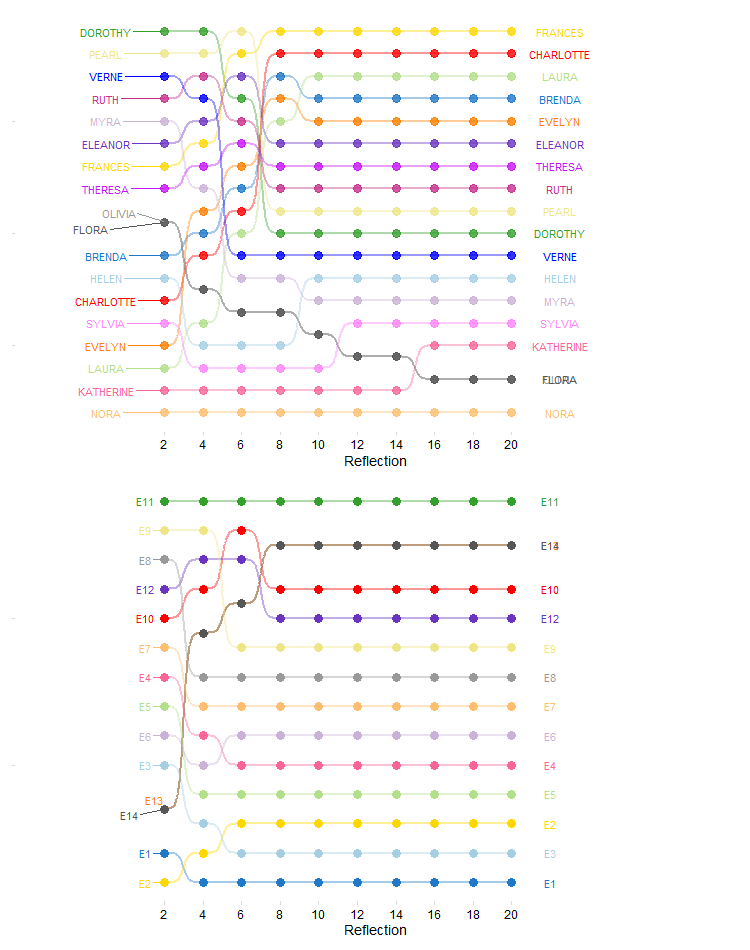
\includegraphics[width=0.75\textwidth]{Plots/pg-reflections.jpg}
    \caption{Reflective centrality trajectories of persons and groups (even reflections).}
    \label{fig:pg-reflections}
\end{figure}

\section{Correspondence Analysis, Dual Centrality, and Communities in Two-Mode Networks} \label{sec:ca}
The reader may ask what the point of going through all these reflective centralities, since \citet{bonacich1991simultaneous} already developed a dual conception of centrality in two-mode networks based on a very similar idea: Define the centralities of entities in one mode based on the centralities of entities in the other mode to which they are connected. In that paper, Bonacich also considered CA in passing but dismissed its application to centrality rankings. Instead, Bonacich noted that, in analyzing the Southern Women data shown in Table~\ref{tab:southern}, ``[r]ather than centrality, what they [CA scores] seem to capture is membership in the two cliques that attended two different sets of events'' \citeyearpar[164]{bonacich1991simultaneous}. 

As we will see, Bonacich was only half right. Indeed, the CA scores capture a version of ``clique'' (more accurately, community) membership, but they---particularly the first dimension---also capture a version of centrality in the most general sense of ranking nodes based on a meaningful criterion \citep{borgatti2006graph}. In fact, they capture the limit $(q \rightarrow \infty)$ of the reflective centralities discussed in the previous section \citep{mealy2019interpreting}. 

To see this, recall that the solutions to the following system of linear equations give the Bonacich $(C^B)$ two-mode centralities:

\begin{equation}
    AC^B_p = \lambda C^B_g 
    \label{eq:bon1}
\end{equation}

\begin{equation}
    A^TC^B_g = \lambda C^B_p 
    \label{eq:bon2}
\end{equation}

Where $A$ is the original affiliation matrix. Equations~\ref{eq:bon1} and~\ref{eq:bon2} have the typical form of a linear eigensystem, which means the unknown $C^B_g$ and $C^B_p$ scores can be obtained from the row and column eigenvectors corresponding to the largest eigenvalue $\lambda$, obtained from the singular value decomposition (SVD) of the rectangular affiliation matrix $A$. Importantly, as Faust \citeyearpar[170]{faust1997centrality} notes, it is possible to express Equations~\ref{eq:bon1} and~\ref{eq:bon2} in terms of person and group-specific centralities. 

For people, these are given by: 

\begin{equation}
    C^B_p = \frac{1}{\lambda}\sum_{g}a_{pg}C^B_g
    \label{eq:faust1}
\end{equation}

And for groups:

\begin{equation}
    C^B_g = \frac{1}{\lambda}\sum_{p}a_{pg}C^B_p
    \label{eq:faust2}
\end{equation}

Where $\lambda$ is the (first) eigenvalue corresponding to the eigenvector containing the $C^B_p$ scores. These equations make clear that in the Bonacich two-mode, the centrality of people is proportional to the centralities of the groups they join, and the centrality of groups is proportional to the centralities of their members. These capture the duality property since the centralities of nodes in each mode are given by aggregating their connections to nodes in the other mode. Note the formal similarity between equations~\ref{eq:faust1} and~\ref{eq:faust2} and equations~\ref{eq:Rq_p} and~\ref{eq:Rq_g}. The main difference is that in the reflective equations, a person's centrality is proportional to the \textit{activity-weighted} centralities of the groups they join, and a group's centrality is proportional to the \textit{group size weighted} centrality of the people who are members. We will return to this crucial point later.

\subsection{The Bonacich Two-Mode Centrality as a Reflective Centrality} \label{subsec:bonref}
To see the connection between the reflective and Bonacich two-mode centralities more clearly, we can motivate the Bonacich two-mode centrality using the same ``reflective'' approach we used to introduce the HH reflective centrality in Section~\ref{sec:ref2mode}. Admittedly, this is a somewhat unorthodox way of presenting the eigenvector centrality for two-mode networks~\citep{bonacich1991simultaneous}, but it will help clarify the similarities and differences between the HH and the Bonacich approaches. Accordingly, starting with Equations~\ref{eq:R1_p} and~\ref{eq:R1_g}, we can define a second-order ``Bonacich-reflection'' on both the persons and groups using the formulas:

\begin{equation}
   C^B_p(2) = \sum_g a_{pg}C^R_g(1)
   \label{eq:BR2_p}
\end{equation} 

\begin{equation}
   C^B_g(2) = \sum_p a_{pg}C^R_p(1)
   \label{eq:BR2_g}
\end{equation}

Equation~\ref{eq:BR2_p} says that people are central when the sum of the number of members of the groups they belong to is large. Equation~\ref{eq:BR2_g} says groups are central when the sum of the number of memberships of the people who belong to them is large. 

As before, we can keep on going and define a third-order reflection using the formulas:

\begin{equation}
   C^B_p(3) = \sum_g a_{pg}C^R_g(2)
   \label{eq:BR3_p}
\end{equation} 

\begin{equation}
   C^B_g(3) = \sum_p a_{pg}C^R_p(2)
   \label{eq:BR3_g}
\end{equation}

Equation~\ref{eq:BR3_p} says that people are central when the sum of the sum of the number of memberships held by the people who belong to the groups they belong to is large. Equation~\ref{eq:BR3_g} says that groups are central when the sum of the sum of the number of members of the groups their members belong to is large. Once again, we can keep going and define fourth order, fifth order, and higher reflections $C^R_p(4), C^R_p(4) \ldots C^R_p(q)$, where the centralities of nodes in one mode are based on the sums, of the sums, of the sums, of the centralities of nodes in the other mode.

More generally, and in parallel with equations~\ref{eq:Rq_p} and~\ref{eq:Rq_g}, the reflective Bonacich centralities for persons and groups are given by:

\begin{equation}
   C^B_p(q) = \sum_g a_{pg}C^R_g(q-1)
   \label{eq:BRq_p}
\end{equation} 

\begin{equation}
   C^B_g(q) = \sum_p a_{pg}C^R_p(q-1)
   \label{eq:BRq_g}
\end{equation} 

This just says that the Bonacich reflective centrality at step $q$ is just the sum of the group centralities at step $q-1$ (for people) and the sum of the person centralities at step $q-1$ (for groups). 

Of course, it is evident that these sum of sums would diverge to a bigger and bigger quantity at each step $q$. To prevent this and guarantee convergence, we normalize the vector of reflective Bonacich centralities for persons and groups at each step $q > 1$ before calculating the subsequent sum at step $q+1$ as follows:

\begin{equation}
   C^B_p(q) = \frac{C^B_p(q)}{||C^B_p(q)||_2}
   \label{eq:BRq_pn}
\end{equation} 

\begin{equation}
   C^B_g(q) = \frac{C^B_g(q)}{||C^B_g(q)||_2}
   \label{eq:BRq_gn}
\end{equation} 

Where the denominator in~\ref{eq:BRq_pn} and~\ref{eq:BRq_gn} is the Euclidean vector norm.\footnote{For any vector $\mathbf{x}$ of length $n$, the $L_2$ norm is given by: $||\mathbf{x}||_2 = \sqrt{\sum_i^n x_i^2}$.} The normalization will prevent divergence of the sum of centralities for persons and groups, formalizing the weaker assumption of \textit{proportionality} between the centrality of each set of nodes and the sum of the centralities of the nodes in the other mode to which they are connected rather than the stronger assumption of strict equivalence \citep{bonacich_lloyd01}. Furthermore, the normalization guarantees convergence and the ``freezing'' of the sums around steady values after a few iterations. These values will be equivalent (up to rounding error) to the (absolute value) of the dominant row and column eigenvectors of $\mathbf{A}$ as given in~\ref{eq:bon1} and~\ref{eq:bon2}.\footnote{Note that dividing by any vector norm---e.g., the $L_1$ or max norm---will prevent divergence and return scores perfectly correlated to the Bonacich eigenvector approach. Dividing by the $L_2$ norm returns scores that are \textit{exactly} the same, save for rounding error, as the absolute value of the dominant left and right eigenvectors of the affiliation matrix.} In fact, the iterative (normalized sum of sums) approach is one way of computing the leading eigenvectors of a rectangular matrix (e.g., the ``power'' method of \citet{mises1929praktische}). 

This exercise establishes that there is more than a superficial similarity between the HH ``reflective'' centralities and the Bonacich two-mode centralities. In fact, both can be seen as instantiating an underlying reflective model of how centrality is distributed in the two-mode network, with the Bonacich approach presuming that centrality points are distributed equally across nodes in each mode regardless of their own centrality (both large and small degree nodes distribute the same ``amount'' of centrality to others) and the HH reflective approach normalizing by the centrality of nodes in each mode, so that nodes distribute a given centrality quantum that is proportional to their first-order degree centrality, with large degree nodes having less centrality to distribute than low degree nodes. 

\subsection{HH Reflective Centrality as an Eigenvector Centrality} \label{subsec:refeigen}
Since iterating through normalized sums of sums is one way of obtaining the Bonacich two-mode centralities, it would be surprising if the equilibrium values of the HH reflective iterations were not themselves the solution to some eigenvalue decomposition problem. As has been noted recently by \citet{mealy2019interpreting} and \citet{van2021correspondence}, the Hidalgo and Hausmann's \citeyearpar{hidalgo2009building} reflective centralities can indeed be obtained directly (without iterations) as the solution to an eigenvalue decomposition problem. 

To see this, recall that, as Bonacich \citeyearpar[157]{bonacich1991simultaneous} notes, we can solve for $C^B_g$ in~\ref{eq:bon2} and $C^B_p$ in~\ref{eq:bon1} and substitute the respective solutions into \ref{eq:bon1} and~\ref{eq:bon2}. Matrix-algebraic reduction of the resulting equations would show that the Bonacich dual centralities can also be obtained as solutions to the eigensystem:

\begin{equation}
    \left(AA^T\right)C^B_p = \lambda^2 C^B_p
    \label{eq:bon3}
\end{equation}

\begin{equation}
    \left(A^TA\right)C^B_g = \lambda^2 C^B_g
    \label{eq:bon4}
\end{equation}

This shows that the dual centrality Bonacich scores for persons and groups are equivalent to the eigenvectors of the respective one-mode projection matrices corresponding to the first (largest) eigenvalue. 

Now, consider the $|P| \times |P|$ matrix $Dp$, which contains the ``first order'' reflective centralities of each person $C^R(1)_p$ (activity) along the diagonals and zeroes in every other cell. In the same way, consider the $|G| \times |G|$ matrix $Dg$, which contains the ``first order'' (degree) centralities of each group $C^R(1)_g$ (size) along the diagonals and zeroes in every other cell. It can be shown \citep{van2021correspondence}, that in the limit ($q \rightarrow \infty$), the iterative HH reflective centralities can be obtained as the solution of the eigensystem:

\begin{equation}
    \left(Dp^{-1}ADg^{-1}A^T\right)C^R_p = \lambda C^R_p
    \label{eq:dam1}
\end{equation}

\begin{equation}
    \left(Dg^{-1}A^TDp^{-1}A\right)C^R_g = \lambda C^R_g
    \label{eq:dam2}
\end{equation}

Note the formal similarity (and key differences) between these equations and the Bonacich two-mode centralities in equations~\ref{eq:bon3} and~\ref{eq:bon4}. Both extract individual and group centralities as eigenvectors of the one-mode projection of the original affiliation matrix: $AA^T$ for people and $A^TA$ for groups. The difference is that the reflective centralities pre-multiply the affiliation matrix and its transpose by the inverse of the first-order centralities of the nodes in each mode before computing the eigenvalue decomposition, essentially normalizing the one-mode projection by the degrees of both sets of nodes. 

This can be clearly seen if we express $\left(Dg^{-1}A^TDp^{-1}A\right)$ in~\ref{eq:dam1} in terms of each cell entry \cite[eq. 4]{mealy2019interpreting}:

\begin{equation}
    a_{pp'} = \sum_g\frac{a_{pg}a_{p'g}}{C^R_p(1)C^R_g(1)} = 
    \frac{1}{C^R_p}\sum_g\frac{a_{pg}a_{p'g}}{C^R_g(1)}
    \label{eq:mealy1}
\end{equation}

In equation~\ref{eq:mealy1}, the numerator is equal to one when person $p$ and person $p'$ share membership in a group $g$. Summed across groups, this gives the number of memberships that $p$ and $p'$ have in common \citep{breiger1974duality}. As noted, the Bonacich dual centralities are obtained from the eigenvector corresponding to the first eigenvalue of this matrix of shared memberships (for people) and shared people (for groups). The reflective centralities, on the other hand, are given by the eigenvectors of a weighted version of the same matrix, where the weights are the sizes of each of the groups $p$ shares with each other person summed across groups and divided by the total number of $p$'s memberships. 

The same reasoning applies to groups in~\ref{eq:dam2}, whose entries are given by:

\begin{equation}
    a_{gg'} = \sum_p\frac{a_{pg}a_{pg'}}{C^R_p(1)C^R_g(1)} = 
    \frac{1}{C^R_g}\sum_p\frac{a_{pg}a_{pg'}}{C^R_p(1)}
    \label{eq:mealy2}
\end{equation}

Now, as has been noted by two-mode data analysts in other contexts \citep[e.g.,][]{faust2005using} it turns out that this ``double-pre-weighting'' of each cell entry by the degrees of each mode (e.g., the row and column sums of the original affiliation matrix) is precisely that used for the CA of a two-mode matrix.\footnote{More accurately, cells are weighted by the inverse of the square root of the product of the row, and column sums \citep[e.g.,][124]{faust2005using}.} And indeed, the limit reflective centralities obtained from equations~\ref{eq:dam1} and~\ref{eq:dam2}---which will be given by the eigenvectors corresponding to the \textit{second} largest eigenvalue of the resulting solution---will be equivalent to the row and column scores corresponding to the first non-trivial dimension (for people and groups respectively) obtained from a simple CA of the original affiliation matrix \citep[398, eq. 9.17]{fouss2016algorithms}.\footnote{As \citet[126]{faust2005using} notes, the first non-trivial CA dimension is also given by the eigenvector corresponding to the second-largest eigenvalue of $D_p^{-1/2}AD_g^{-1/2}$.} In fact, the method of ``reflections'' is just a re-discovery of the older idea of reciprocal averaging \citep{hill1973reciprocal}, which is yet another way of computing row and column scores for elements in a two-mode matrix that are substantively equivalent to those obtained by (the first non-trivial dimension of) CA \citep{mealy2019interpreting}.

Degree-pre-weighting does not radically alter the nature of the data. Indeed, it corresponds to moving from sums to averages, thus ``adjusting'' for the influence of person-activity and group size---a seemingly perennial issue in two-mode data analysis \citep[159ff]{bonacich1991simultaneous}. This can be seen by the fact that Equations~\ref{eq:mealy1} and~\ref{eq:mealy2} show that, substantively, what the degree pre-weighting does is that, for people, co-memberships count for more in determining interpersonal similarity when the group in question is small than when it is large. On the group side, shared members who do not have many affiliations count more in determining intergroup similarity than those with many affiliations. 

Accordingly, it would make no sense to call the Bonacich scores $C^B_p$ and $C^B_g$ from equations~\ref{eq:bon3} and~\ref{eq:bon4} ``centrality scores'' but fail to hold that designation from $C^R_p$ and $C^R_g$, given that the mathematics are not only ``similar'' \citep[162]{bonacich1991simultaneous} but formally identical. In the Bonacich case, an eigendecomposition of the one-mode projection of the two-mode network; in the reflective case, an eigendecomposition of the degree-weighted one-mode projection of the same network. Accordingly, the CA of a two-mode network will return---along the first dimension---a rank-ordered score for nodes in each mode that meets all the conditions for qualifying as a centrality measure for two-mode networks. Particularly, the CA centrality retains the duality property \citep[128]{faust2005using}, as the (average) centrality of people is a function of the (average) centrality of the groups they belong to. The (average) centrality of groups, in turn, is a function of their members' (average) centrality. The person and group score ranks given by the first CA dimension are thus better thought of as \textit{activity and group-size normalized} versions of the familiar Bonacich \citeyearpar{bonacich1991simultaneous} dual centralities for two-mode networks.

\begin{figure}
    \centering
    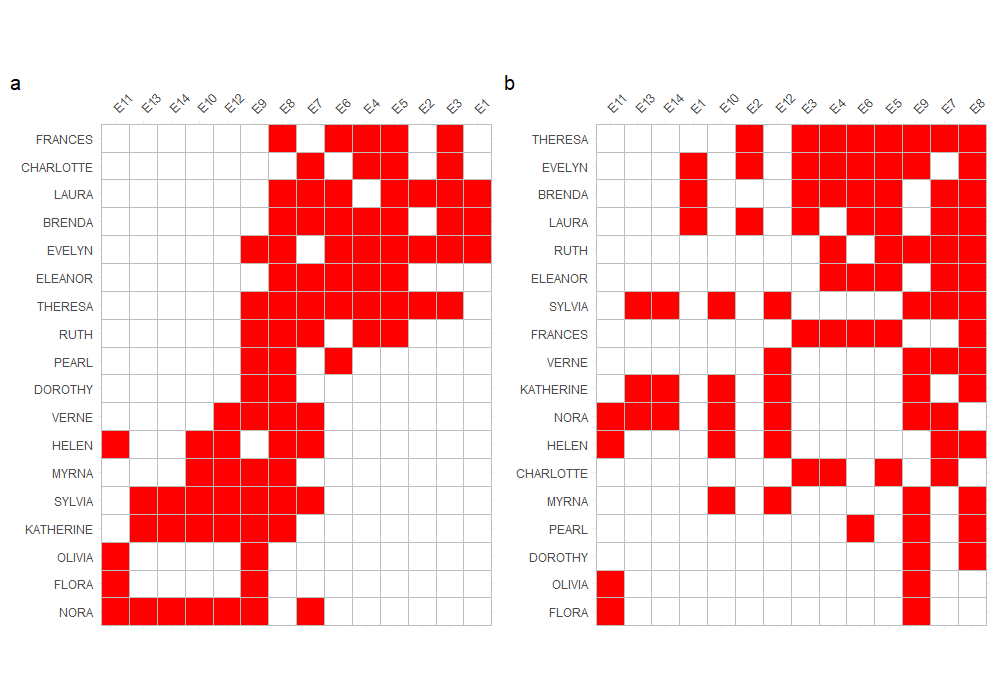
\includegraphics[width=0.8\textwidth]{Plots/ca-v-bon-reord.png}
    \caption{Southern Women Affiliation matrix with re-ordered rows and columns: (a) row and columns re-ordered according to the person and group score on the first CA dimension, (b) row and columns re-ordered according to person and group Eigenvector centrality score.}
    \label{fig:ca-v-bon}
\end{figure}

\section{Illustrative Analysis of the Southern Women Data} \label{sec:anal}
\subsection{Row and Column Re-ordered Affiliation Matrices}
Figures~\ref{fig:ca-v-bon}(a) and~\ref{fig:ca-v-bon}(b) illustrate the key differences between the two versions of dual centrality $C^R$ and $C^B$. Each panel shows the original Southern Women affiliation matrix but with rows and columns re-ordered according to the first CA dimension in (a) and the \citet{bonacich1991simultaneous} centrality in (b). In the plot, a cell entry is colored red if it has a one in the original affiliation matrix and is white when the corresponding entry is zero. As we can see, the two row-column-reshuffled matrices have appreciably distinct structures, with the $C^R$ re-ordered affiliation matrix having a block-diagonal structure and the $C^B$ re-ordered affiliation matrix having a triangular structure. Accordingly, the $C^R$ centrality rankings reveal a dual community partition between groups of women who selectively attend two groups of events (on the top-right and bottom-left of the plot). The traditional eigenvector centrality re-ordering, on the other hand, reveals a classic core-periphery partitioning \citep{borgatti2000models}, with a group of highly active women (on the top-left) who selectively co-participate in highly attended events (on the top right-hand side of the plot) and less active women (in the bottom half) who go to less well-attended events (on the left side). The two centralities extract qualitatively different information from the two-mode network, with $C^R$ geared toward community partitioning and $C^B$ more focused on finding a core of well-connected people and groups. 

\subsection{Eigenvector Plot} \label{subsec:eigplot}
We can confirm that the first CA axis points toward the underlying community partitioning of the two-mode network by looking at Figure~\ref{fig:ca-eigvec}(a) and~\ref{fig:ca-eigvec}(c), which shows the $C^R$ score of persons and groups on the x-axis against the score's rank order on the y-axis. If a two-mode network has no discernible community structure, the first dimension CA scores would be distributed as a continuous logistic curve; when community structure is present, we should observe discernible breaks in this distribution \citep{van2021correspondence}. The Southern Women data clearly belong to the second category. In the people mode, we have $\left[Frances, Laura, Brenda, Charlotte, Evenly, Theresa, Elanor, Ruth, Pearl\right]$ on one side, $\left[Dorothy, Nora, Katherine, Sylvia, Flora, Olivia, Myra, Helen, Verne\right]$ on the other. Among events, we have $\left[E1, E2, E3, E4, E5, E6\right]$ on side $\left[E9, E10, E11, E12, E13, E14\right]$ on the other and $\left[E7, E8\right]$ in an ambiguous middle position. Note that this is roughly the same partitioning obtained by \citep{doreian2004generalized} and reproduced by \citet{kovacs2010generalized} and \citet{lizardo2024two} using a generalized relational similarity approach. This indicates that persons and groups receive similar scores in the first dimension of CA only when they have similar connectivity similar to \textit{similar} groups, where group similarity is defined dually as having members in common who are themselves similar. 

\begin{figure}
    \centering
    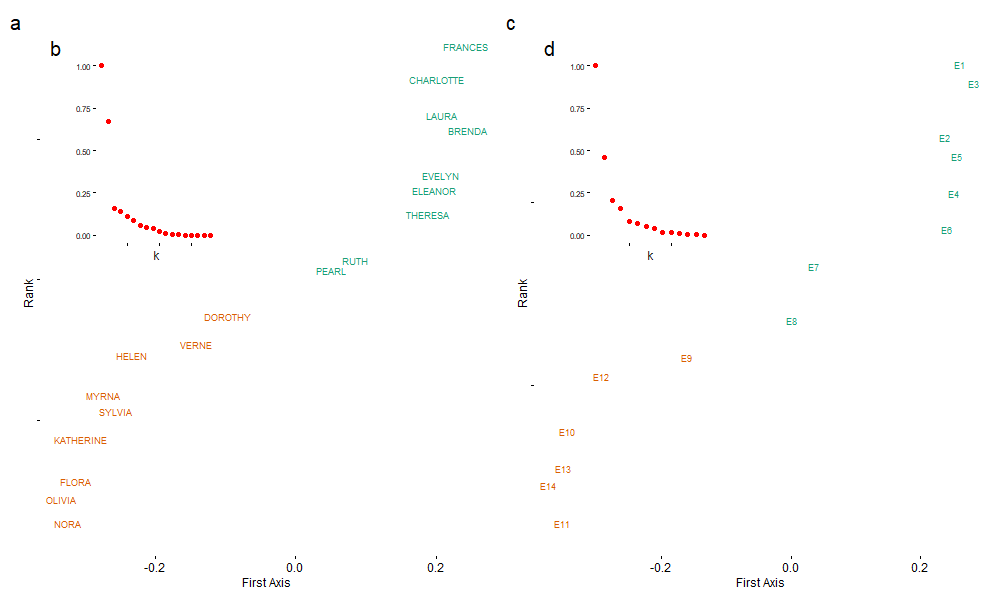
\includegraphics[width=0.8\textwidth]{Plots/ca-eigvec.png}
    \caption{CA Eigenvector plot for persons (a) and groups (c). The first CA score is on the x-axis, and the rank order of persons and groups is on the y-axis. Insets show the eigenvalue orderings on the x-axis ($k$) for persons (b) and groups (d).}
    \label{fig:ca-eigvec}
\end{figure}

\subsection{Normalized Similarity Plot} \label{subsec:normsim}
To further appreciate the links between CA, reflective centralities, and community partitioning in two-mode networks, note that $S_p = ADg^{-1}A^T$ in~\ref{eq:dam1} can be thought of as giving the similarity between pairs of people weighted by the size of the groups they belong to (so that people are more similar when they share smaller memberships).\footnote{Note that \citet[eq.2]{newman2001scientific} proposes a slightly modified version of this two-mode similarity score for people---in Newman's case, scientists---except that the one mode projection is normalized as $A(Dg - I)^{-1}A^T$; namely, the size of the ``group''---the number of co-authors on a scientific paper---minus one. Substantively, this is unlikely to make much difference as the rank order of dyads by similarity between the two scores will be identical.} The same interpretation can be given to $S_g = A^TDp^{-1}A$ in~\ref{eq:dam2}, which is the similarity of groups weighted by the activity of the people in them (so that groups are more similar when they share members who do not belong to many other groups). As \citet{van2021correspondence} show, the eigenvectors corresponding to (the Laplacian\footnote{For the similarity matrix $S$, the Laplacian is defined as $D-S$ where $D$ is the matrix containing the degrees of either people or groups in the diagonal and zeroes in every other cell.} of) these similarity matrices are equivalent to $C^R$. This means that the relative spread of the eigenvalues of the degree-weighted similarity matrix provides information concerning the quality of the resulting community partition. These are shown as inset plots in Figure~\ref{fig:ca-eigvec} for both people and groups. Note that in both cases, the first two eigenvalues separate from the rest, strongly indicating a dual-community structure in the Southern Women two-mode network. 

\begin{figure}
    \centering
    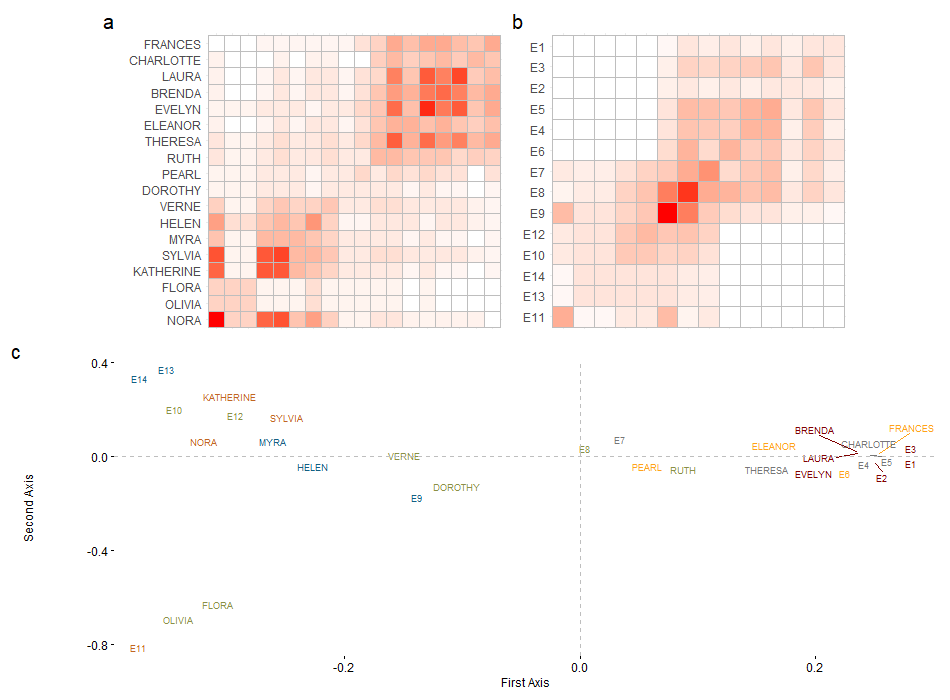
\includegraphics[width=1.0\textwidth]{Plots/ca-sim.png}
    \caption{CA similarity plots for persons (a) and groups (b) on the left and right top panel. The bottom panel (c) shows the correspondence plot for persons and groups with scores corresponding to the first dimension on the horizontal axis and scores corresponding to the second dimension on the vertical axis.}
    \label{fig:ca-sim}
\end{figure}

To fix the intuition, the top-left panel (a) of Figure~\ref{fig:ca-sim} shows a heatmap representation of the group-size weighted similarity matrix $S_p$ (for people); the top-right panel (b) shows the same plot for the activity-weighted similarity matrix $S_g$ (for groups). In both figures, darker squares indicate more similar node pairs, and closer to white indicate less similarity. Moreover, the rows of each matrix are sorted according to $C^R$ for both people and groups. As we can see, for both people and groups, the re-ordered matrix recovers maximally similar communities of nodes, where the similarity is based on their shared (degree-weighted) connections to entities in the other mode. 

\subsection{CA Correspondence Plot} \label{subsec:caplot}
The bottom panel of Figure~\ref{fig:ca-sim} shows the usual correspondence plot of the first two CA dimensions. People and groups are colored according to a six-cluster k-means solution based on the first nine eigenvectors of their respective similarity matrices. The plot reveals that the distances between nodes in the standard correspondence plot---usually taken to be a low-dimensional representation of the \textit{original} affiliation matrix \citep{borgatti1997network}---are best thought of as low-dimensional representations of the (other mode's) degree-normalized similarity network across people and groups. People with similar values in $S_p$---such as $\left[Olivia, Flora\right]$,  $\left[Katherine, Sylvia, Nora\right]$, $\left[Dorothy, Verne\right]$, and $\left[Brenda, Laura, Evelyn\right]$--- appear closer in the correspondence plot (and are assigned to the same cluster by the k-means algorithm). The same goes for events, those with similar values in $S_g$---such as $\left[E13, E14\right]$ and $\left[E1, E2, E3\right]$---appear closer in the correspondence plot, while those with dissimilar values are placed far apart. The distances between same-mode entities in the correspondence plot will thus be a function of their (inverse) degree-normalized similarity.

Note that this differs from the usual interpretation of the CA correspondence plot, which is usually taken to bring together nodes with ``similar'' connectivity patterns, where similarity is presumed to be a function of their raw row profiles (for people) or column profiles (for groups). This interpretation implies (for instance) that two people who attend many of the same events or two groups with many members will appear close in the plot. But this (still common) interpretation is off the mark. What the CA correspondence plot distance captures is, instead, people and groups that are \textit{surprisingly} similar (e.g., from the point of view of a suitable null model, like independence) after taking people's activity levels and the sizes of the groups they belong to into account.\footnote{Note that this, finding ``surprising'' similarities in terms of the indirect paths linking nodes in a network after the main effects of node-connectivity are considered, is the same rationale given by \cite{leicht2006vertex} for weighting the \citet{katz1953new} similarity matrix by the degrees of the corresponding nodes \citep[see][68, eqs. 2.13 and 2.14]{fouss2016algorithms}. As we have seen, this is precisely the key contrast between the Bonacich and the CA dual centrality measures for two-mode networks.} Thus, people who share memberships in small groups will be closer in the diagram than people who share memberships in big groups. In the same way, groups that share people with few memberships will be closer in the diagram than those sharing people with many other memberships. 

\begin{figure}
    \centering
    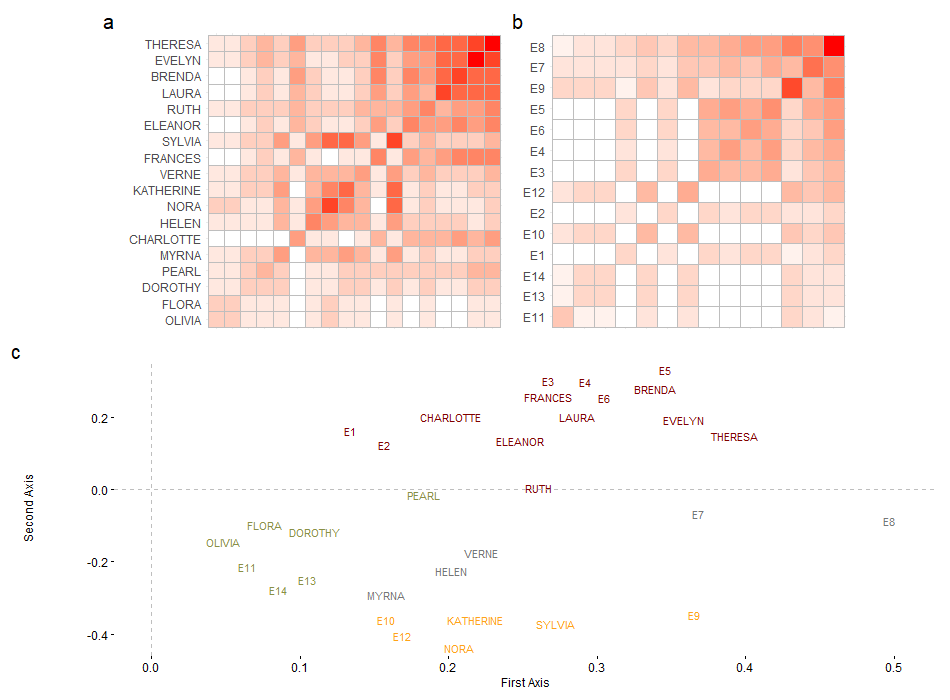
\includegraphics[width=1.0\textwidth]{Plots/bon-sim.png}
    \caption{Bonacich dual centrality similarity plots for persons (a) and groups (b) on the left and right top panel. The bottom panel (c) shows the Bonacich eigenvector centrality correspondence plot for persons and groups with scores corresponding to the standard Bonacich eigenvector centrality on the horizontal axis and scores corresponding to the second largest eigenvector of the affiliation matrix on the vertical axis.}
    \label{fig:bon-sim}
\end{figure}

\subsection{One-Mode Projection Matrix and Eigevenctor Plot}
This ambiguity in interpretation may stem from the fact that CA is usually seen as a technique to generate a plot that provides a ``low-dimensional approximation to the input data'' \citep[125]{faust2005using}, where the ``input data'' is presumed to be the original affiliation matrix $\mathbf{A}$. But as we have seen, this is \textit{not} what CA is designed to do. Instead, CA is meant to provide a low-dimensional approximation of a \textit{transformed} version of the input data, where the transformation is meant to adjust for people's activity levels and group sizes. Notably, if a low-dimensional representation of the original ``input data'' ($\mathbf{A}$) is what we are after, this may be more closely approximated by the first two eigenvectors of the usual one-mode projections of the matrix (where the first is, of course, the standard Bonacich dual centrality score). 

To illustrate, Figures~\ref{fig:bon-sim}(a) and~\ref{fig:bon-sim}(b) shows the ``raw'' (unweighted by other-mode degree) similarity scores for persons ($a_{pp'} = \sum_g a_{pg}a_{p'g}$) and groups ($a_{gg'} = \sum_p a_{pg}a_{pg'}$), with the rows and columns sorted by the first eigenvector of the matrix, which is the usual Bonacich centrality score. Both similarity matrices reproduce the triangular, core-periphery structure we observed in the re-ordered affiliation matrix in Figure~\ref{fig:ca-v-bon}(b).  Figure~\ref{fig:bon-sim}(c) plots $C^B$ on the x-axis against the second eigenvector of the unweighted similarity matrix---a relatively unusual but not substantively unmotivated practice \citep{iacobucci2017eigenvector}.\footnote{Nodes are colored to a four-cluster k-means solution using the first six eigenvectors of the respective similarity matrices.}  We can see that the plot of the first two eigenvectors does a good job of recovering the raw connectivity structure of the Southern Women affiliation network, partitioning the core persons and groups (on the upper-right) from the more peripheral ones (on the lower-left). 

Moreover, if all we are interested in is capturing a low-dimensional representation of which people have particular affinities for which events (regardless of people's activity levels or group sizes), then Figure~\ref{fig:bon-sim}(c) does a better job of that than the usual CA correspondence plot in Figure~\ref{fig:ca-sim}(c). For instance, $\left[Flora, Olivia\right]$ do have a special affinity for $\left[E11\right]$ and $\left[Nora, Katherine, Sylvia\right]$ for $\left[E10, E12\right]$. In the same way, core events like $\left[E8, E9, E10\right]$---shown on the lower half of the plot---are different from core events $\left[E3, E4, E5, E6\right]$---shown in the upper half. The former are more inclusive of peripheral members while the latter are more ``cliquish,'' including only core members. 

This ``preferential attachment'' \citep{barabasi1999emergence} of core people to core events and peripheral people to peripheral events seems to be captured by the second dimension, left over after considering each node's Bonacich eigenvector centrality. For instance, $\left[E1, E2\right]$, although as poorly attended as other peripheral events, tends to include core members and thus appear closer to other core actors in the upper half of the plot. Similarly, the main difference between $\left[Ruth\right]$ and $\left[Sylvia\right]$, despite their comparable $C^B$ scores, is that the former's (closer to the upper half of the plot) event profile is composed mainly of core events. In contrast, peripheral events dominate the latter's attendance profile (shown in the bottom half of the plot), accordingly, $\left[Ruth\right]$ and $\left[Sylvia\right]$ are assigned to distinct clusters by the k-means algorithm. 

\subsection{Correspondence Analysis and Generalized Relational Similarity} \label{subsec:cagensim}
As noted, there seems to be a relationship between the ordering of persons and groups produced by CA of a two-mode network and that produced by previous work using a ``generalized relational similarity'' (GRS) strategy. Recall that for objects (let us say people) to be similar according to the GRS criterion, they must have overlapping connections, and those links should go to objects in the other mode \textit{that are themselves similar}, where objects' similarities are given by their pattern of connections to objects in the other mode. This recursive definition of similarity thus recalls the classic distinction between structural and regular equivalence \citep{everett1994regular}. In the context of two-mode networks, \citet{kovacs2010generalized} proposed one such approach to defining a GRS for nodes in one and two-mode networks using a modified version of the correlation distance.\footnote{\citet{lizardo2024two} shows the connection between Kovacs's idea of generalized relations similarity and the two-mode network projection.}

An earlier effort to define a GRS for persons and groups in two-mode networks, one more relevant for a direct comparison with CA and the ``reflective'' approaches already considered, can be found in \citet{jeh2002simrank}. In that work, the authors dubbed their similarity measure ``SimRank.'' In the context of two-mode network analysis, the goal is to compute a matrix of similarities for each of the two-node sets, where the similarity of people is a function of the groups they belong to, and the similarity of groups is a function of the people who belong to them, making the similarity of persons and groups ``mutually reinforcing notions'' \citep[540]{jeh2002simrank}. Thus,

\begin{itemize}
    \item People are \textit{similar} if they belong to \textit{similar} groups.
    \item Groups are \textit{similar} if they share \textit{similar} members.
\end{itemize}

Which is consistent with a GRS approach \citep[see][]{kovacs2010generalized, lizardo2024two}. To accomplish this, \citet[540, eq. 2 and eq. 3]{jeh2002simrank} propose that we define the similarity of each pair of people $S(p, p')$  as given by:

\begin{equation}
    S(p, p') = \frac{\alpha}{C^R(1)_pC^R(1)_{p'}}
    \sum_{i = 1}^{C^R(1)_p} \sum_{j = 1}^{C^R(1)_{p'}} 
    S\left(g(i)_{i \in N(p)}, g(j)_{j \in N(p')}\right)
    \label{eq:simrank1}
\end{equation}

Where everything is as before, and $g(i)_{i \in N(p)}$ is the $i^{th}$ group in the set of groups that person $p$ belongs to, $g(j)_{j \in N(p')}$ is the $j^{th}$ group in the set of groups that person $p'$ belongs to, and $\alpha$ is a free parameter obeying the restriction: $0 > \alpha < 1$. By construction, $S(p, p) = 1$, for all $p$. Thus, equation \ref{eq:simrank1} says that the SimRank similarity between two people is a function of the sum of the similarities of each unordered pair of groups they both belong to, weighted by the reciprocal of the products of their number of memberships multiplied by $\alpha$.

Likewise, for groups, the SimRank similarities are given by:

\begin{equation}
    S(g, g') = \frac{\alpha}{C^R(1)_gC^R(1)_{g'}}
    \sum_{i = 1}^{C^R(1)_g} \sum_{j = 1}^{C^R(1)_{g'}} 
    S\left(p(i)_{i \in N(g)}, p(j)_{j \in N(g')}\right)
    \label{eq:simrank2}
\end{equation}

Where $p(i)_{i \in N(g)}$ is the $i^{th}$ person in the set of members of group $g$, and $p(j)_{j \in N(g')}$ is the $j^{th}$ person in the set of members of group $g'$, and $S(g, g) = 1$. Thus, the SimRank similarity between two groups is a function of the sum of the similarities of each pair of people who belong to both groups, weighted by the reciprocal of the products of the number of members of each group multiplied by $\alpha$.

\begin{figure}
    \centering
    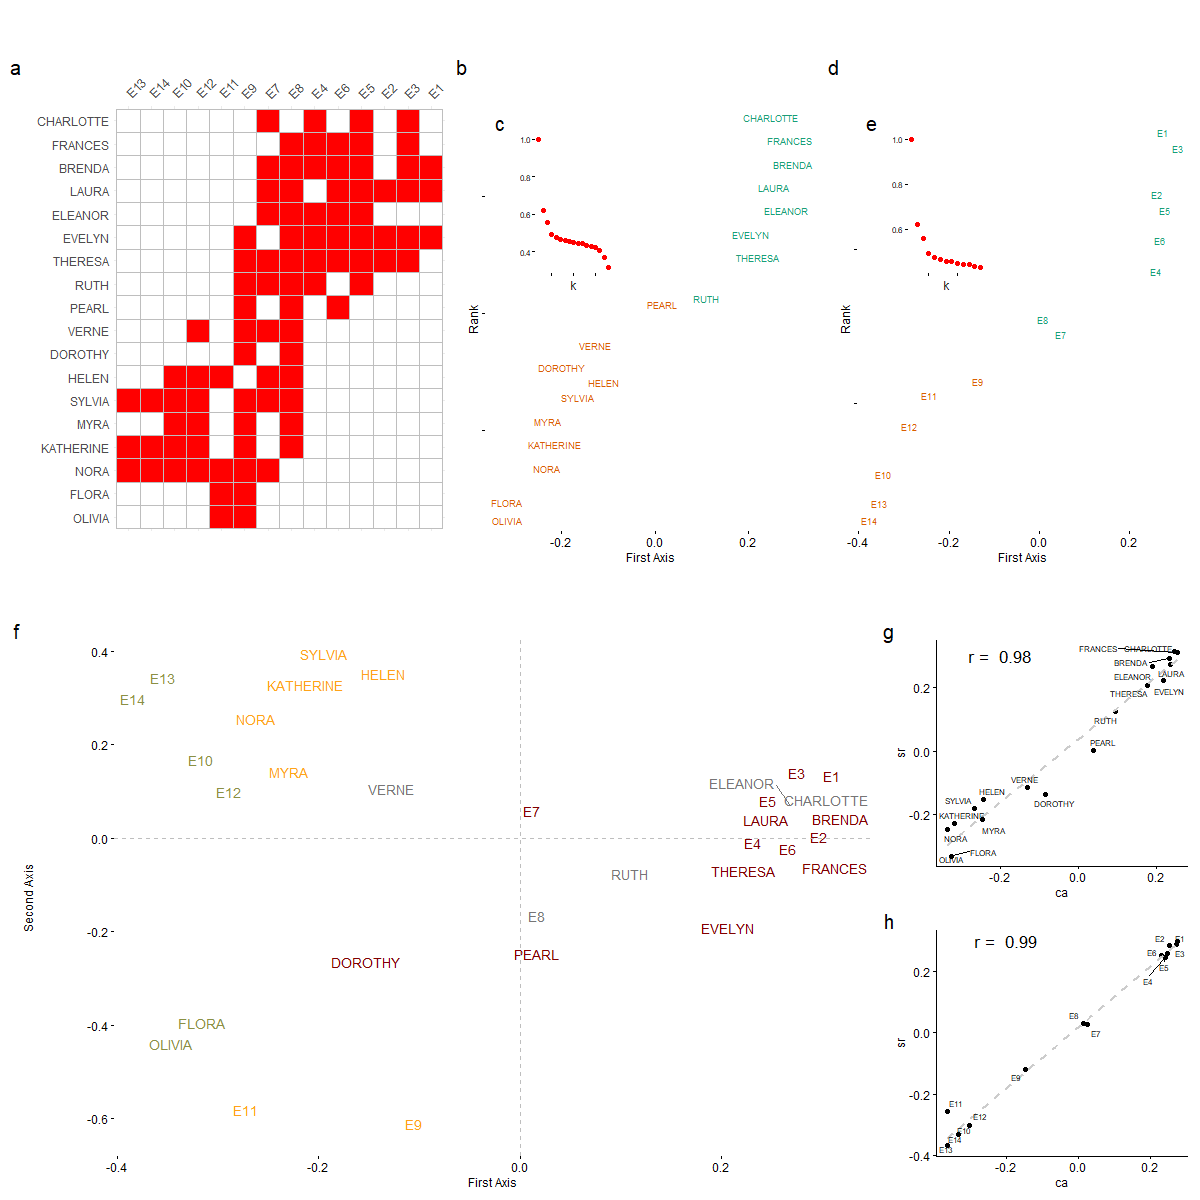
\includegraphics[width=0.8\textwidth]{Plots/sr-plot.png}
    \caption{Simrank versus CA comparison. Panel (a) shows the affiliation matrix re-ordered according to the first eigenvector of the SVD of the SimRank similarity matrix. Panels (b) and (d) show the corresponding eigenvector and eigenvalue---panels (c) and (e)---plots for persons and groups, respectively, of the SimRank similarity matrix. Panel (f) shows the correspondence plot based on the eigenvector decomposition of the SimRank similarity matrix. Panels (g) and (h) show the Pearson correlation between the scores corresponding to the first eigenvector of the SimRank similarity matrix (on the y-axis) and the scores corresponding to the first CA dimension (on the x-axis).}
    \label{fig:simrank}
\end{figure}

In two-mode networks, SimRank scores for each pair of nodes across the two sets can be estimated via a simple algorithm, in which we first estimate $S(p, p')$ in equation \ref{eq:simrank1} using baseline values. Hence, only groups that two people share contribute to the initial values of $S(p, p')$ since only $S(g, g)>0$ at the outset. We then plug those values into equation \ref{eq:simrank2}, then loop back to equation \ref{eq:simrank1} with the resulting $S(g, g')$ values, and continue iterating until convergence---generally achieved after five iterations \citep{jeh2002simrank}, which is confirmed here for the Southern Women data. 

Note that equations~\ref{eq:simrank1} and~\ref{eq:simrank2} share a formal similarity with HH's ``method of reflections'' discussed earlier, in particular, the fact that both compute quantities based on nodes in the other mode averaged by the degree of nodes in the focal mode. The key difference is that SimRank works directly with pairwise comparisons between node dyads \citep{jeh2002simrank}. Nevertheless, this double weighting by degree should make us suspect that the results of the SimRank similarity analysis would not be too far from those obtained via CA, given the mathematical equivalence of CA and the method of reflections \citep{mealy2019interpreting, van2021correspondence}.

And indeed, they are not. Figure~\ref{fig:simrank}(a) shows the original affiliation matrix, this time with rows and columns re-arranged according to the values of the main non-trivial eigenvector (corresponding to the second-largest eigenvalue) of the SimRank similarity matrices---with $\alpha$ set to $0.8$---for the row and column nodes. Like in Figure~\ref{fig:ca-v-bon}(a), this reshuffling reveals the block-diagonal structure separating the two communities of persons and groups revealed by CA, suggesting that CA and SimRank uncover a similar underlying partitioning of the two-mode network's community structure. 

Figure~\ref{fig:simrank}(b) and Figure~\ref{fig:simrank}(d) show a plot similar to that shown in Figures~\ref{fig:ca-eigvec}(a) and Figure~\ref{fig:ca-eigvec}(b) but this time with the main eigenvector of SimRank similarity matrices of both persons and groups on the x-axis and the corresponding rank on the y-axis. Looking at the plots from left to right, we can see that the partitioning of the node sets on the first informative eigenvector is substantively equivalent to those revealed by the first CA eigenvector, separating similar blocks of people and events.  

Figure~\ref{fig:simrank}(f) shows the correspondence plot of the first and second eigenvectors of the SimRank similarity matrices for both persons and groups. Once again, this plot is substantively equivalent (in terms of the internode groupings and distances) to that shown in Figure~\ref{fig:ca-sim}(c), suggesting that the first-CA dimensions of the two-mode network recover clusters of ``similar'' entities in the two node sets, where internode similarity is a generalized relational similarity as defined earlier. Thus, [$Flora, Olivia$] appear close because they choose similar groups, as do [$Sylvia, Katherine, Helen$]. In the same way, groups [$E9, E11$] are close in the plot because they are chosen by similar people, as are events [$E10, E12, E13, E14$]. Figures~\ref{fig:simrank}(g) and (h) show a regression plot of the first CA eigenvector for persons (top) and groups (bottom) on the x-axis and the first eigenvector of the SimRank similarity matrix for both persons and groups on the y-axis. As we can see, the CA and SimRank ordering of nodes along the first dimension agree quite closely ($r = 0.98$ for persons and $r = 0.99$ for groups), confirming that these first eigenvectors capture the same (GSR) information across the two approaches. 

\section{Discussion and Concluding Remarks} \label{sec:disc}
This paper reconsiders the role of CA in the analysis of two-mode network data. We began with an accidental ``rediscovery'' of CA in the analysis of two-mode networks via a ``reflective'' approach \citep{hidalgo2009building}, showing that the method of reflections leads to an eigenvector-style solution that is equivalent to simple CA of the affiliation matrix. Working backward from this, we also clarified the linkages between CA and the more commonly used eigenvector approach for calculating dual centralities in two-mode data due to \citet{bonacich1991simultaneous}. I showed that just like the reflective centralities that converge to the CA scores of the affiliation matrix, we could also think of the Bonacich centralities as the equilibrium solution to reflective iterations through the two-mode matrix, with the main difference being that the CA reflections deal with sums of averages weighted by the degrees of nodes in each mode, while the Bonacich approach works with unweighted (but normalized) sums. This exercise clarifies the links between CA and the dual two-mode eigenvector centrality in a more coherent and systematic way, an issue that was left open and somewhat unclear in Bonacich's (1991) classic paper. Thus, one conclusion that emerges from this analysis is that CA computes a kind of centrality for two-mode networks, equivalent to Hidalgo and Hausman's ``reflective'' centrality \citep{van2021correspondence}.

But CA does more than reveal a latent dual ordering of nodes in the two-mode network. In addition to doing this, CA can be shown to reveal \textit{groupings} of nodes based on some conception of the similarity of their connections to nodes in the other mode. This is evident once we use the scores of the first CA dimension to re-order the rows and columns of the original affiliation matrix. When the CA scores are used, a clear (and now well-known) dual partition between persons and groups emerges in the classic Southern Women data. This partition is substantively distinct from that which would emerge if we use the same approach to re-ordering the original data using the Bonacich centralities, which instead uncover a latent core-periphery partition between actors and events. 

This is another way in which CA and the Bonacich dual centrality approach systematically differ; one is geared to uncovering blocks of actors with similar connections to events in the other mode (and vice versa), while the other reveals blocks of actors who are the most active and who attend the largest events. Both are, of course, legitimate ways of analyzing the structure of a two-mode network. Still, they differ in terms of the structural patterns that they are sensitive to, with the CA approach closer to a community partition where nodes that are surprisingly similar end up in the same clusters---where ``surprising'' means similarity based on deviations from a suitable null model based on random mixing given their first-order degrees. 

But what kind of similarity is the clustering based on the CA of the two-mode network sensitive to? Here we argued that CA recovers a type of generalized relational similarity (GRS). That is, actors who have similar patterns of linkage to similar events are deemed similar, while events that have similar patterns of connectivity to similar actors are also deemed similar. Using a well-known iterative method to recover such generalized similarities from two-mode networks \citep{jeh2002simrank}, we saw that the scores from the first dimension of CA end up being a fairly accurate approximation to the resulting partition from the generalized relational similarity approach. Thus, we can clarify that two-mode network CA reveals latent groupings of nodes based on a GRS criterion. 

Overall, the preceding has shown that CA can be upgraded from a method designed to generate joint plots and visualization of two-mode data to one that can be seen as more ``central'' to the usual social-network-analytic tasks, like ordering the nodes in the two sets according to some substantively meaningful rank---centrality analysis---or finding sets of similar actors in the network (subgroup or community detection). At the very least, it seems like the Bonacich style dual centrality based on the eigenvector decomposition of the raw affiliation matrix should not be the default ``reflective'' centrality approach unless the analyst has the explicit analytic goal of exploring center-periphery partitioning in the network. 

A better approach, similar to the one exemplified here, would be to present a comparison of the reflective centralities obtained by CA and Bonacich side-by-side to see whether the underlying display a substantively interesting similarity partitioning in addition to any core-periphery ordering. Of course, suppose the analyst is more interested in such a ``subgroup'' analytic approach. In that case, the Bonacich dual centrality approach is less helpful (even if multiple dimensions are considered), and CA should be the first line of attack. 



%% Loading bibliography style file]
%\bibliographystyle{model1-num-names}
\bibliographystyle{cas-model2-names}
% Loading bibliography database
\bibliography{ca.bib}
\end{document}


The Elsevier cas-dc class is based on the
standard article class and supports almost all of the functionality of
that class. In addition, it features commands and options to format the
\begin{itemize} \item document style \item baselineskip \item front
matter \item keywords and MSC codes \item theorems, definitions and
proofs \item labels of enumerations \item citation style and labeling.
\end{itemize}

This class depends on the following packages
for its proper functioning:

\begin{enumerate}
\itemsep=0pt
\item {natbib.sty} for citation processing;
\item {geometry.sty} for margin settings;
\item {fleqn.clo} for left aligned equations;
\item {graphicx.sty} for graphics inclusion;
\item {hyperref.sty} optional packages if hyperlinking is
  required in the document;
\end{enumerate}  

All the above packages are part of any
standard \LaTeX{} installation.
Therefore, the users need not be
bothered about downloading any extra packages.

\section{Installation}

The package is available at author resources page at Elsevier
(\url{http://www.elsevier.com/locate/latex}).
The class may be moved or copied to a place, usually,\linebreak
\verb+$TEXMF/tex/latex/elsevier/+, %$%%%%%%%%%%%%%%%%%%%%%%%%%%%%
or a folder which will be read                   
by \LaTeX{} during document compilation.  The \TeX{} file
database needs updation after moving/copying class file.  Usually,
we use commands like \verb+mktexlsr+ or \verb+texhash+ depending
upon the distribution and operating system.

\section{Front matter}

The author names and affiliations could be formatted in two ways:
\begin{enumerate}[(1)]
\item Group the authors per affiliation.
\item Use footnotes to indicate the affiliations.
\end{enumerate}
See the front matter of this document for examples. 
You are recommended to conform your choice to the journal you 
are submitting to.

\section{Bibliography styles}

There are various bibliography styles available. You can select the
style of your choice in the preamble of this document. These styles are
Elsevier styles based on standard styles like Harvard and Vancouver.
Please use Bib\TeX\ to generate your bibliography and include DOIs
whenever available.

Here are two sample references: 
\cite{Fortunato2010}
\cite{Fortunato2010,NewmanGirvan2004}
\cite{Fortunato2010,Vehlowetal2013}

\section{Floats}
{Figures} may be included using the command,\linebreak 
\verb+\includegraphics+ in
combination with or without its several options to further control
graphic. \verb+\includegraphics+ is provided by {graphic[s,x].sty}
which is part of any standard \LaTeX{} distribution.
{graphicx.sty} is loaded by default. \LaTeX{} accepts figures in
the postscript format while pdf\LaTeX{} accepts {*.pdf},
{*.mps} (metapost), {*.jpg} and {*.png} formats. 
pdf\LaTeX{} does not accept graphic files in the postscript format. 

\begin{figure}
	\centering
		\includegraphics[scale=.75]{figs/Fig1.pdf}
	\caption{The evanescent light - $1S$ quadrupole coupling
	($g_{1,l}$) scaled to the bulk exciton-photon coupling
	($g_{1,2}$). The size parameter $kr_{0}$ is denoted as $x$ and
	the \PMS is placed directly on the cuprous oxide sample ($\delta
	r=0$, See also Table \protect\ref{tbl1}).}
	\label{FIG:1}
\end{figure}


The \verb+table+ environment is handy for marking up tabular
material. If users want to use {multirow.sty},
{array.sty}, etc., to fine control/enhance the tables, they
are welcome to load any package of their choice and
{cas-dc.cls} will work in combination with all loaded
packages.

\begin{table}[width=.9\linewidth,cols=4,pos=h]
\caption{This is a test caption. This is a test caption. This is a test
caption. This is a test caption.}\label{tbl1}
\begin{tabular*}{\tblwidth}{@{} LLLL@{} }
\toprule
Col 1 & Col 2 & Col 3 & Col4\\
\midrule
12345 & 12345 & 123 & 12345 \\
12345 & 12345 & 123 & 12345 \\
12345 & 12345 & 123 & 12345 \\
12345 & 12345 & 123 & 12345 \\
12345 & 12345 & 123 & 12345 \\
\bottomrule
\end{tabular*}
\end{table}

\section[Theorem and ...]{Theorem and theorem like environments}

{cas-dc.cls} provides a few shortcuts to format theorems and
theorem-like environments with ease. In all commands the options that
are used with the \verb+\newtheorem+ command will work exactly in the same
manner. {cas-dc.cls} provides three commands to format theorem or
theorem-like environments: 

\begin{verbatim}
 \newtheorem{theorem}{Theorem}
 \newtheorem{lemma}[theorem]{Lemma}
 \newdefinition{rmk}{Remark}
 \newproof{pf}{Proof}
 \newproof{pot}{Proof of Theorem \ref{thm2}}
\end{verbatim}


The \verb+\newtheorem+ command formats a
theorem in \LaTeX's default style with italicized font, bold font
for theorem heading and theorem number at the right hand side of the
theorem heading.  It also optionally accepts an argument which
will be printed as an extra heading in parentheses. 

\begin{verbatim}
  \begin{theorem} 
   For system (8), consensus can be achieved with 
   $\|T_{\omega z}$ ...
     \begin{eqnarray}\label{10}
     ....
     \end{eqnarray}
  \end{theorem}
\end{verbatim}  


\newtheorem{theorem}{Theorem}

\begin{theorem}
For system (8), consensus can be achieved with 
$\|T_{\omega z}$ ...
\begin{eqnarray}\label{10}
....
\end{eqnarray}
\end{theorem}

The \verb+\newdefinition+ command is the same in
all respects as its \verb+\newtheorem+ counterpart except that
the font shape is roman instead of italic.  Both
\verb+\newdefinition+ and \verb+\newtheorem+ commands
automatically define counters for the environments defined.

The \verb+\newproof+ command defines proof environments with
upright font shape.  No counters are defined. 


\section[Enumerated ...]{Enumerated and Itemized Lists}
{cas-dc.cls} provides an extended list processing macros
which makes the usage a bit more user friendly than the default
\LaTeX{} list macros.   With an optional argument to the
\verb+\begin{enumerate}+ command, you can change the list counter
type and its attributes.

\begin{verbatim}
 \begin{enumerate}[1.]
 \item The enumerate environment starts with an optional
   argument `1.', so that the item counter will be suffixed
   by a period.
 \item You can use `a)' for alphabetical counter and '(i)' 
  for roman counter.
  \begin{enumerate}[a)]
    \item Another level of list with alphabetical counter.
    \item One more item before we start another.
    \item One more item before we start another.
    \item One more item before we start another.
    \item One more item before we start another.
\end{verbatim}

Further, the enhanced list environment allows one to prefix a
string like `step' to all the item numbers.  

\begin{verbatim}
 \begin{enumerate}[Step 1.]
  \item This is the first step of the example list.
  \item Obviously this is the second step.
  \item The final step to wind up this example.
 \end{enumerate}
\end{verbatim}

\section{Cross-references}
In electronic publications, articles may be internally
hyperlinked. Hyperlinks are generated from proper
cross-references in the article.  For example, the words
\textcolor{black!80}{Fig.~1} will never be more than simple text,
whereas the proper cross-reference \verb+\ref{tiger}+ may be
turned into a hyperlink to the figure itself:
\textcolor{blue}{Fig.~1}.  In the same way,
the words \textcolor{blue}{Ref.~[1]} will fail to turn into a
hyperlink; the proper cross-reference is \verb+\cite{Knuth96}+.
Cross-referencing is possible in \LaTeX{} for sections,
subsections, formulae, figures, tables, and literature
references.

\section{Bibliography}

Two bibliographic style files (\verb+*.bst+) are provided ---
{model1-num-names.bst} and {model2-names.bst} --- the first one can be
used for the numbered scheme. This can also be used for the numbered
with new options of {natbib.sty}. The second one is for the author year
scheme. When  you use model2-names.bst, the citation commands will be
like \verb+\citep+,  \verb+\citet+, \verb+\citealt+ etc. However when
you use model1-num-names.bst, you may use only \verb+\cite+ command.

\verb+thebibliography+ environment.  Each reference is a\linebreak
\verb+\bibitem+ and each \verb+\bibitem+ is identified by a label,
by which it can be cited in the text:

\noindent In connection with cross-referencing and
possible future hyperlinking it is not a good idea to collect
more that one literature item in one \verb+\bibitem+.  The
so-called Harvard or author-year style of referencing is enabled
by the \LaTeX{} package {natbib}. With this package the
literature can be cited as follows:

\begin{enumerate}[\textbullet]
\item Parenthetical: \verb+\citep{WB96}+ produces (Wettig \& Brown, 1996).
\item Textual: \verb+\citet{ESG96}+ produces Elson et al. (1996).
\item An affix and part of a reference:\break
\verb+\citep[e.g.][Ch. 2]{Gea97}+ produces (e.g. Governato et
al., 1997, Ch. 2).
\end{enumerate}

In the numbered scheme of citation, \verb+\cite{<label>}+ is used,
since \verb+\citep+ or \verb+\citet+ has no relevance in the numbered
scheme.  {natbib} package is loaded by {cas-dc} with
\verb+numbers+ as default option.  You can change this to author-year
or harvard scheme by adding option \verb+authoryear+ in the class
loading command.  If you want to use more options of the {natbib}
package, you can do so with the \verb+\biboptions+ command.  For
details of various options of the {natbib} package, please take a
look at the {natbib} documentation, which is part of any standard
\LaTeX{} installation.

\appendix
\section{My Appendix}
Appendix sections are coded under \verb+\appendix+.

\verb+\printcredits+ command is used after appendix sections to list 
author credit taxonomy contribution roles tagged using \verb+\credit+ 
in frontmatter.

\printcredits




%\vskip3pt

\bio{}
Author biography without author photo.
Author biography. Author biography. Author biography.
Author biography. Author biography. Author biography.
Author biography. Author biography. Author biography.
Author biography. Author biography. Author biography.
Author biography. Author biography. Author biography.
Author biography. Author biography. Author biography.
Author biography. Author biography. Author biography.
Author biography. Author biography. Author biography.
Author biography. Author biography. Author biography.
\endbio

\bio{figs/pic1}
Author biography with author photo.
Author biography. Author biography. Author biography.
Author biography. Author biography. Author biography.
Author biography. Author biography. Author biography.
Author biography. Author biography. Author biography.
Author biography. Author biography. Author biography.
Author biography. Author biography. Author biography.
Author biography. Author biography. Author biography.
Author biography. Author biography. Author biography.
Author biography. Author biography. Author biography.
\endbio

\bio{figs/pic1}
Author biography with author photo.
Author biography. Author biography. Author biography.
Author biography. Author biography. Author biography.
Author biography. Author biography. Author biography.
Author biography. Author biography. Author biography.
\endbio

